\documentclass[12pt, a4paper, oneside]{article}
%die Pakete werden hier durch den Include-Befehl separat eingelesen
\usepackage[utf8]{inputenc}
\usepackage{amsmath} % Mathematik-Pakete
\usepackage{amsfonts}
%\usepackage{mathptmx} %times new roman
%\usepackage[T1]{fontenc} %vollen Zeichensatz ]
\usepackage{amssymb}
\usepackage[ngerman]{babel}
\usepackage{graphicx}
\usepackage{microtype} %besserer Randausgleich
\usepackage{footnote}
\usepackage{blindtext}
\usepackage{etoolbox}
%\usepackage{makeidx}
%\usepackage{dsfont}
\usepackage{lettrine}%\usepackage{geometry}
%\usepackage{xcolor} % Für verschiedene Farben
\newcommand{\ricardo}[1]{\colorbox{ForestGreen}{\color{white}   \textsf{\textbf{Ricardo}}} \textcolor{ForestGreen}{#1}}
\usepackage[pdfborderstyle={/S/U/W 1}]{hyperref} % Für interaktive Refernzierung im PDF
\usepackage{csquotes}
\usepackage{acro}
\usepackage{hyperref} % Für interaktive Refernzierung im PDF
\usepackage[onehalfspacing]{setspace}%Zeilenabstand 1.5
% \usepackage{picins} % Das Umfließen einer Grafik im Text kann mit dem Paket PicIns erreicht werden.
%\usepackage{fontspec} 

%\usepackage[utf8]{inputenc}
\usepackage[ngerman]{babel}
\usepackage[top=2.5cm, bottom=2.5cm, left=2cm, right=3.5cm]{geometry}
\usepackage{bibgerm}
\usepackage{tabularx}
\usepackage{adjustbox}
\usepackage{cite}
\usepackage{blindtext}
\usepackage{epsfig}
\usepackage{longtable}
%\usepackage{showframe}
\usepackage{dcolumn}%benötigt für stargaze
\usepackage{here}%lädt das Paket zum Erzwinge n der Grafikposition
\usepackage{floatflt}%Bilder im Fließtext
%\usepackage{fontspec}
%\usepackage{fontenc}
\usepackage{dsfont}
%\setsansfont[Ligatures=TeX]{Arial}
%\renewcommand{\familydefault}{\sfdefault}
%\usepackage{times}
\usepackage{graphicx}
\usepackage{epstopdf}

\usepackage{xcolor}
\usepackage{listings}

\usepackage{lipsum}




\lstset{language=R}
\lstset{basicstyle=\ttfamily,
basicstyle=\small}
\lstset{literate=%
  {Ö}{{\"O}}1
  {Ä}{{\"A}}1
  {Ü}{{\"U}}1
  {ß}{{\ss}}1
  {ü}{{\"u}}1
  {ä}{{\"a}}1
  {ö}{{\"o}}1
}

\title{\textbf{Titel der Arbeit}}
\author{Max Mustermann}

\setlength{\parindent}{0cm} %keine Einrückung
\linespread{1.5} 

\acsetup{first-style=short}
\newpage


\newpage
%in alphabetischer Reihenfolge

\newcounter{SeitenzahlSpeicher}
\begin{document}

 \thispagestyle{empty}
\begin{titlepage}
	 \thispagestyle{empty}
	% thispagestyle{empty} unterdrückt Seitenzahlen auf der gewünschten Seite
	\newfont{\smc}{cmcsc10 at 12pt}
%	\maketitle
	%Aufpassen mit fi: Fehlercode U+FB01
	%%%%%%%%%%%%%%%%%%%%%%%%%%%%%%%%%%%%%%%%%%
%Titel, Autor, Seminar, Semester, Dozent %
%%%%%%%%%%%%%%%%%%%%%%%%%%%%%%%%%%%%%%%%%%
\begin{center}
	 \thispagestyle{empty}
\begin{figure}[t]
	\centering
	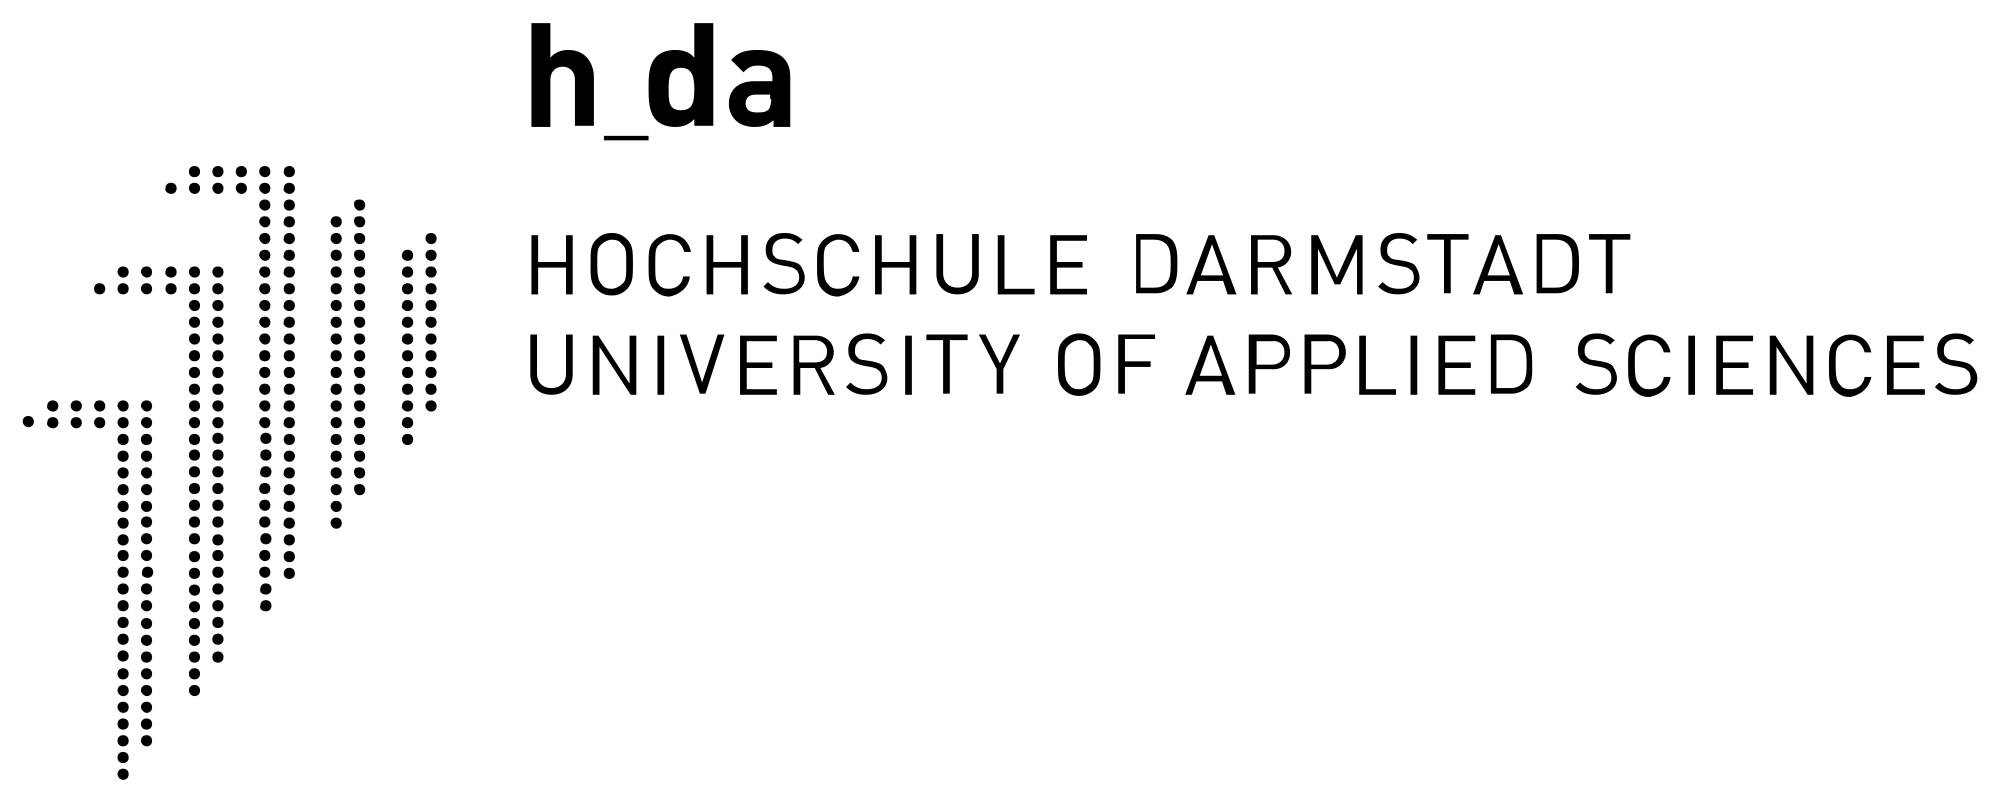
\includegraphics[width=0.6\textwidth]{Hda_logo.svg.png}
	
\end{figure}

$~~$\\
\paragraph{}$~~$\\
\paragraph{}$~~$\\
\textbf{\huge Projektdokumentation eFinder}\paragraph{}$~~$\\
\paragraph{}$~~$\\
\paragraph{}$~~$\\
\textbf{im Rahmen des Fachs Nutzerzentrierte Softwareentwicklung}\\ \textbf{am Fachbereich Informatik}\\ \textbf{der Hochschule Darmstadt}
\paragraph{}$~~$\\
\paragraph{}$~~$\\
\paragraph{}$~~$\\
\paragraph{}$~~$\\
\text{von: Lukas Räpple \& Etienne Gotha}\\
\text{Dozent: Prof. Dr. Hans-Peter Wiedling}\\
\end{center}	
\end{titlepage}



\begin{spacing}{1}
\pagenumbering{Roman}
\setcounter{page}{2}
\tableofcontents
\end{spacing}
\newpage
\begin{spacing}{1}
\section*{Abbildungsverzeichnis} 
\addcontentsline{toc}{section}{Abbildungsverzeichnis}
\renewcommand{\listfigurename}{}
\listoffigures
\end{spacing}
\newpage
\clearpage
\setcounter{SeitenzahlSpeicher}{\value{page}}
\pagenumbering{arabic}
\newpage
\pagenumbering{arabic}

\section{Einführung}
\subsection{Projektbeschreibung}


\subsection{Vorgehensweise}
%Gang der Untersuchung:
%-Vorgehensweise
%-Auf Kapitel beziehen

\section{Entwurf}
\subsection{User Story Mapping}
\subsection{Prototyping}
\subsection{Softwaredesign}

\section{Entwicklung}
\subsection{Navigationsleiste}
\subsection{Registrierung \& Login}
\subsubsection{Datenbankintegration}
\subsection{Map-Screen}
\subsubsection{Google-Maps Integration}
\subsection{Such-Screen}
\subsection{Admin-Screen}
\subsection{Favoriten-Screen}
\subsection{Einstellungs-Screen}

\section{Testen}
\subsection{Funktionale Tests}
\subsection{Usability-Test}
\newpage

\section{Fazit}

\section{Literaturverzeichnis}
\bibliographystyle{gerplain}
\renewcommand{\refname}{} 
\bibliography{bibba}

\newpage


\appendix %Anhang
\pagenumbering{arabic}
\section{Anhang}

\newpage

\section{Eigenständigkeitserklärung}
``Ich versichere, dass ich die Arbeit selbständig und ohne Benutzung anderer als der angegebenen Hilfsmittel angefertigt habe. Alle Stellen, die wörtlich oder sinngemäß aus Veröffentlichungen oder anderen Quellen entnommen sind, sind als solche kenntlich gemacht. Die schriftliche und die elektronische Form der Arbeit stimmen überein. Ich stimme der Überprüfung der Arbeit durch eine Plagiatssoftware zu.''
\paragraph{}$~~$\\
\paragraph{}$~~$\\
\vspace{50pt} 
\noindent\rule{5cm}{.4pt}\hfill\rule{5cm}{.4pt}\par 
\noindent Ort, Datum \hfill Unterschrift 
\end{document}